\section{Combinations without repetition}

In combinations, order does not matter. We are interested only in which objects are selected, not in the order in which they are written.

This is a different way of thinking from permutations and variations. In an ordered list, \(ab\) and \(ba\) are different. In an unordered selection, they represent the same choice. The objects are collected into a group, not placed into positions.

\begin{definitionbox}
Let \(A\) be a finite set with \(n\) distinct elements, and let \(k\leq n\). A combination without repetition of size \(k\) is a \(k\)-element subset of \(A\).
\end{definitionbox}

For example, if
\[
A=\{a,b,c\},
\]
then the combinations without repetition of size \(2\) are
\[
\{a,b\},\qquad \{a,c\},\qquad \{b,c\}.
\]
The expressions \(\{a,b\}\) and \(\{b,a\}\) describe the same set, so they are not counted separately.

\begin{center}
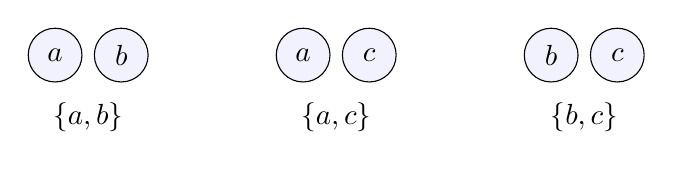
\begin{tikzpicture}[scale=1.05, transform shape]
\foreach \first/\second/\x in {a/b/0, a/c/3, b/c/6} {
    \node[draw, circle, fill=blue!5, minimum size=0.65cm] at (\x,0) {$\first$};
    \node[draw, circle, fill=blue!5, minimum size=0.65cm] at (\x+0.8,0) {$\second$};
    \node at (\x+0.4,-0.75) {$\{\first,\second\}$};
}
\end{tikzpicture}
\end{center}

\begin{theorembox}
The number of combinations without repetition of size \(k\) chosen from \(n\) distinct elements is
\[
\binom{n}{k}=\frac{n!}{k!(n-k)!}.
\]
\end{theorembox}

To see why, first count ordered selections without repetition. There are
\[
V(n,k)=\frac{n!}{(n-k)!}
\]
of them. But each unordered group of \(k\) elements can be ordered in \(k!\) ways. Therefore each combination has been counted \(k!\) times. Dividing by \(k!\) gives
\[
\frac{1}{k!}\cdot \frac{n!}{(n-k)!}=\frac{n!}{k!(n-k)!}.
\]

This division by \(k!\) is not a trick. It removes the internal orderings of the same selected group.

\begin{examplebox}
From six distinct books, choose three books to take on a trip. The order of choosing does not matter. The number of possible selections is
\[
\binom{6}{3}=\frac{6!}{3!3!}=20.
\]
\end{examplebox}

\begin{examplebox}
From the set \(\{1,2,3,4,5\}\), choose two numbers. The possible groups are not ordered, so \(\{1,4\}\) and \(\{4,1\}\) are the same group. The number of choices is
\[
\binom{5}{2}=10.
\]
\end{examplebox}

\begin{remarkbox}
Use combinations without repetition when order does not matter and no object may be selected more than once. Typical words are: choose, select, form a group, form a committee, pick a subset.
\end{remarkbox}
